\documentclass{beamer}

\begin{filecontents}{ref.bib}
    @article{mckenney2017parallel,
    title={Is Parallel Programming Hard, And, If So, What Can You Do About It?(Release v2022. 09.25 a)},
    author={McKenney, Paul E},
    journal={arXiv preprint arXiv:1701.00854},
    year={2017}
    }
    @inproceedings{schwaricke2021real,
    title={A real-time virtio-based framework for predictable inter-VM communication},
    author={Schw{\"a}ricke, Gero and Tabish, Rohan and Pellizzoni, Rodolfo and Mancuso, Renato and Bastoni, Andrea and Zuepke, Alexander and Caccamo, Marco},
    booktitle={2021 IEEE Real-Time Systems Symposium (RTSS)},
    pages={27--40},
    year={2021},
    organization={IEEE}
    }
    @inproceedings{struhr,
    author =	{V{\'a}clav Struh{\'a}r and Moris Behnam and Mohammad Ashjaei and Alessandro V. Papadopoulos},
    title =	{{Real-Time Containers: A Survey}},
    booktitle =	{2nd Workshop on Fog Computing and the IoT (Fog-IoT 2020)},
    year =	{2020},
    }
    @inproceedings{barletta2022achieving,
    title={Achieving isolation in mixed-criticality industrial edge systems with real-time containers},
    author={Barletta, Marco and Cinque, Marcello and De Simone, Luigi and Della Corte, Raffaele},
    booktitle={34th Euromicro Conference on Real-Time Systems (ECRTS 2022)},
    year={2022},
    organization={Schloss Dagstuhl-Leibniz-Zentrum f{\"u}r Informatik}
    }
    @inproceedings{abranches2019shimmy,
    title={Shimmy: Shared memory channels for high performance inter-container communication},
    author={Abranches, Marcelo and Goodarzy, Sepideh},
    booktitle={USENIX Workshop on Hot Topics in Edge Computing (HotEdge)},
    year={2019}
    }
    @inproceedings{dechev2006lock,
    title={Lock-free dynamically resizable arrays},
    author={Dechev, Damian and Pirkelbauer, Peter and Stroustrup, Bjarne},
    booktitle={OPODIS},
    volume={4305},
    pages={142--156},
    year={2006},
    organization={Springer}
    }
    @inproceedings{yun2013memguard,
    title={Memguard: Memory bandwidth reservation system for efficient performance isolation in multi-core platforms},
    author={Yun, Heechul and Yao, Gang and Pellizzoni, Rodolfo and Caccamo, Marco and Sha, Lui},
    booktitle={2013 IEEE 19th Real-Time and Embedded Technology and Applications Symposium (RTAS)},
    pages={55--64},
    year={2013},
    organization={IEEE}
    }
\end{filecontents}


\usepackage{wrapfig}
\usepackage{algpseudocode}
\usepackage{algorithm}
\usepackage[export]{adjustbox}
\usepackage{svg}
\usepackage{multirow}

\usetheme{Boadilla}
\usecolortheme{dolphin}
\setbeamertemplate{navigation symbols}{}
\setbeamertemplate{sections/subsections in toc}[sections numbered]

\title[VM and Container Communications]{Shared Memory Process Communication in VM and Container Hosts}
\author[Afkar]{Hossein Afkar}
\institute{University of Tehran}
\date{\today}

\begin{document}

\frame{\titlepage}

\begin{frame}
    \frametitle{Table of Contents}
    \tableofcontents[hideallsubsections]
\end{frame}

% 1. Talk about the importance of communication
% 2. Talk about how real-time community and industry 4.0 needs reliable communication
% 3. Containers vs VMs
% 4. What do we need
% 5. Memory bandwidth our focus
% 6. MemGuard
% 7. Achieving control on memory regions how should we do it
% 8. VirtIO how it can help us
% 9. io_uring how can it help
% 10. DRAM ranks and cache coloring
% 11. Memory Ordering
% 12. Lock freedom
% 13. Our Design for container communication
% 14. shared memory implementation
% 15. Conclusion and Future works

\section{Introduction and Motivation}

\begin{frame}
    \frametitle{Why We Need Inter Process Communication}
    \begin{itemize}
        \item Collaboration between processes.
        \item Distributed Computing.
        \item Security and isolation.
        \item Integral Part of the micro-kernel and exo-kernel design.
    \end{itemize}
\end{frame}

\begin{frame}
    \frametitle{Importance of Communication in Industry 4.0}
    Industry 4.0 refers to the integration of advanced technologies,
    such as automation, data analytics, and the Internet of Things,
    to create smart, interconnected, and highly efficient industrial
    systems. This measn that:
    \begin{itemize}
        \item Distributed systems are present.
        \item Many computing nodes are present
            \begin{itemize}
                \item Need for consolidating computing nodes.
                \item Virtualization is key.
                \item Containers and VMs should be deterministic.
            \end{itemize}
        \item Communication is key.
    \end{itemize}
\end{frame}

\begin{frame}
    \frametitle{Containers vs VMs}
    Use cases vary by much but features are desired in many applications \\
    \begin{table}[ht]
        \centering
        \begin{tabular}{|p{0.4\textwidth}|p{0.4\textwidth}|} \hline
            Virtual Machines & Containers \\ \hline
            Kernel and various resourses are virtualized, High overhead
            & Kernel is shared as a resource. Lowers the overhead \\ \hline
            High isolation & Subpar resource isolation \\ \hline
            Startup time is kernel and userland & Only userland \\ \hline
            Does not rely on host os & Relies on host os \\ \hline
            Hypervisor managed & Kernel managed \\ \hline
        \end{tabular}
        \caption{Comparing containers and virtual machines}
    \end{table}
\end{frame}

\begin{frame}
    \frametitle{Our Goals}
    \begin{itemize}
        \item Consolidate various ECUs used in Industry 4.0.
        \item Tackle communications between units present in the same
            host that were seperated before.
        \item Fast and not marshalled solution for local tenants.
        \item No contention on the memory bus.
        \item No contention on locks.
        \item Bound the memory access latency.
    \end{itemize}
    We will focus on shared memory and memory bandwidth reservation methods.
\end{frame}

\section{Achieve Memory Bandwidth Control}

\begin{frame}
    \frametitle{MemGuard: What it Tries to Fix}
    \begin{itemize}
        \item Memory bandwidth is a highly variable resource in multi-core
            systems.
        \item Applications may create contention on the shared memory bus.
        \item MemGuard paper implemented a fast memory bandwidth reservation
            system. \cite{yun2013memguard}
        \item It performs on the PMCs recieved from each cpu core.
        \item Isolation achieved by this method is a great compliment to
            mixed-critical systems.
            \begin{itemize}
                \item Highly dependent on Intels PMCs.
                \item Not aware of memory regions.
                \item Not aware of the underlying memory architecture
                    (DRAM ranks and cache).
            \end{itemize}
    \end{itemize}
\end{frame}

\begin{frame}
    \frametitle{Controlling Memory Regions: Is It Possible?}
    Overall memory accesses are possible by using PMCs. \\
    Dont Cross the kernel boundary.
    \begin{itemize}
        \item Trap on memory region, High Overhead.
        \item Kernel software trace points (perf and events), High Overhead.
        \item Hardware trace points, Not real-time.
        \item Process signaling, High Overhead.
        \item Userlevel bookkeeping, Lower Overhead, Accurate?
    \end{itemize}
\end{frame}

\begin{frame}
    \frametitle{VirtIO as A Shared Memory Space in VMs}
    This approach was discussed in \cite{schwaricke2021real}
    \begin{itemize}
        \item VirtIO is a virtualization standard for network and disk device
            drivers where just the guest's device driver "knows" it is running
            in a virtual environment, and cooperates with the hypervisor.
        \item Not part of Xen but standardizes Xens approach.
        \item Uses ring buffers like the Xen.
        \item Use it to create a shared space for VMs.
        \item How to make it deterministic?
            \begin{itemize}
                \item Control bandwidth \cite{yun2013memguard}.
                \item Use cache and page coloring.
                \item Don't share VMs between multiple cpu core.
            \end{itemize}
    \end{itemize}
\end{frame}

\begin{frame}
    \frametitle{io\_uring: Asynchronous System Calls}
    io\_uring is an interface for asynchronous system calls in linux kernel. \\
    \begin{itemize}
        \item Works by employing two ring buffers.
        \item Ring buffers are prevalent in network adapters and in most
            designs that rely on single producer and single consumer.
        \item Recently it has been enabled for network system calls.
        \item Asynchronous subsystem calls for correct scheduling inside
            kernel.
        \item High performance because of zero copy design.
    \end{itemize}
\end{frame}

\begin{frame}
    \frametitle{Cache or Page Coloring: Is It Required?}
    \begin{itemize}
        \item Allocate physical pages that are contiguous from the cpu cache
            point of view.
        \item Makes memory access times more deterministic (Not all the way.).
        \item Implemented in NT kernel and FreeBSD but not Linux.
        \item Xen supports cache coloring for VMs.
        \item Together with DRAM rank awareness it becomes a required
            system model for memory determinism.
    \end{itemize}
\end{frame}

\begin{frame}
    \frametitle{Achieving Lock Freedom: Memory Ordering and Hardware Tools}
    Atomic Primitves are provided by the hardware.
    \begin{itemize}
        \item Load-Linked \& Store-Conditional.
        \item Fences.
        \item Compare And Exchange.
    \end{itemize}
    Memory models are provided by the hardware and exploited by programming
    languages.
    \begin{itemize}
        \item Sequencial Consistency.
        \item Weak Ordering.
        \item Total Store Ordering.
    \end{itemize}
    But models are not limited to these most architectures have their own
    ordering That should be studied like the Intel memory ordering paper.
\end{frame}

\begin{frame}
    \frametitle{C++ Memory Models}
    Memory\_order enum describes how the atomic functions should behave with
    regards to the memory model.
    \begin{itemize}
        \item seq\_qst: sequential consistency that we expect.
        \item consume: order the loads with loads and writes to the
            same address so that no loads or writes can happen before.
        \item acquire: order the loads with loads and writes to the
            any address so that no loads or writes can happen before.
        \item release: order the stores with loads and writes to the
            any address so that no loads or writes can happen before.
        \item acquire/release: sum of the two above.
        \item relaxed: No memory ordering enforced.
    \end{itemize}
    One of the challenges in this section is how to use this model in formal
    methods more info can be found in  \cite{mckenney2017parallel}.
\end{frame}

\begin{frame}
    \frametitle{Lock Freedom: Types of Non Blocking Algorithms}
    Non blocking algoritms can be categorized into following classification.
    \begin{description}[Obstruction Freedom]
        \item[Obstruction Freedom] Means that we gurantee progress as long
            there is no contention between thread.
        \item[Lock Freedom] Adds the requirement that the system as a whole
            makes progress even if there is contention.
        \item[Wait Freedom] Adds the requirement that every thread makes
            progress even if meets contention.
    \end{description}
    \cite{dechev2006lock} proposed a design for a lock free vector
    implementation. \\
\end{frame}

\begin{frame}
    \frametitle{CASVector vs Mutex}
    \begin{figure}
        \centering
        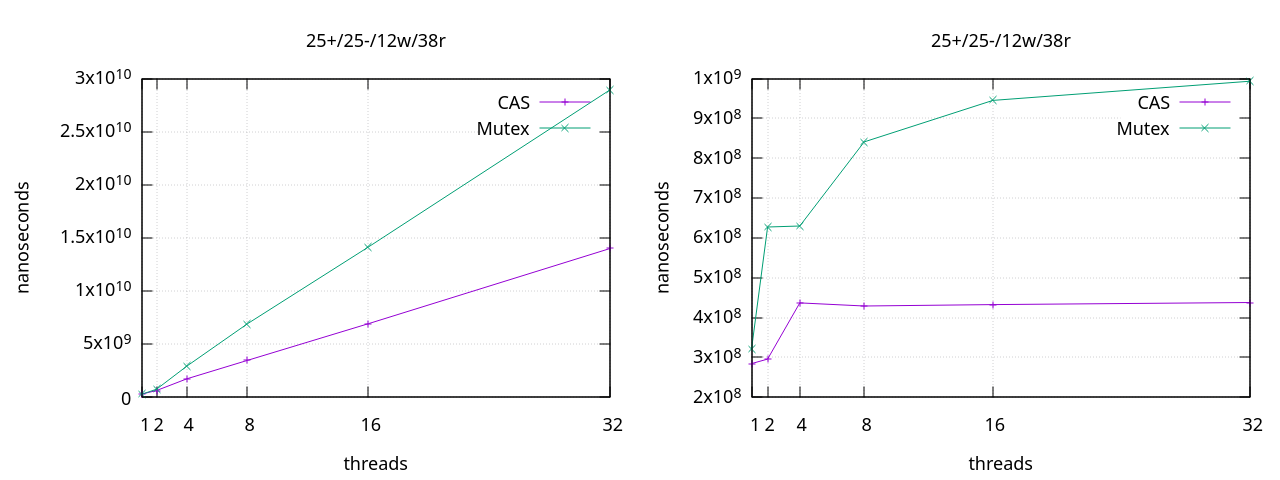
\includegraphics[width=1.0\textwidth]{res.png}
        \caption{Mutex vs CAS Vector}
        \label{fig:res}
    \end{figure}
\end{frame}


\section{Propose a Design}

\begin{frame}
    \frametitle{Proposed Design for Container Communication}
    \begin{figure}
        \centering
        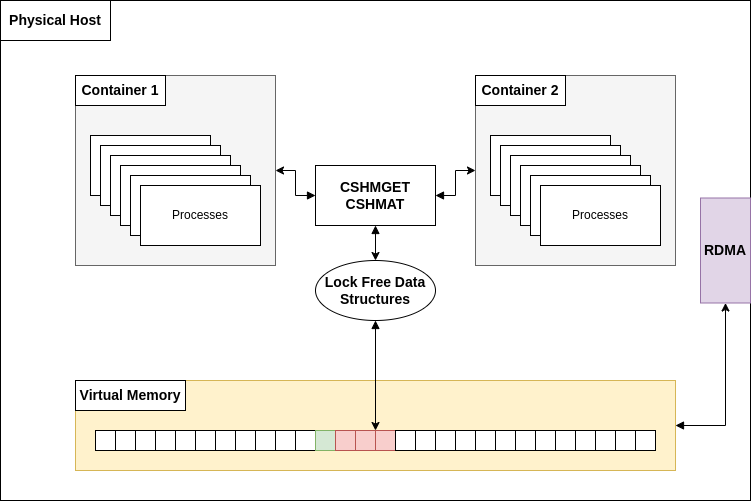
\includegraphics[width=0.8\textwidth]{dist.png}
        \caption{Simple Architecture Of The Proposed Design: Kernel Based}
        \label{fig:desg}
    \end{figure}
\end{frame}

\begin{frame}
    \frametitle{Proposed Design for Container Communication}
    \begin{figure}
        \centering
        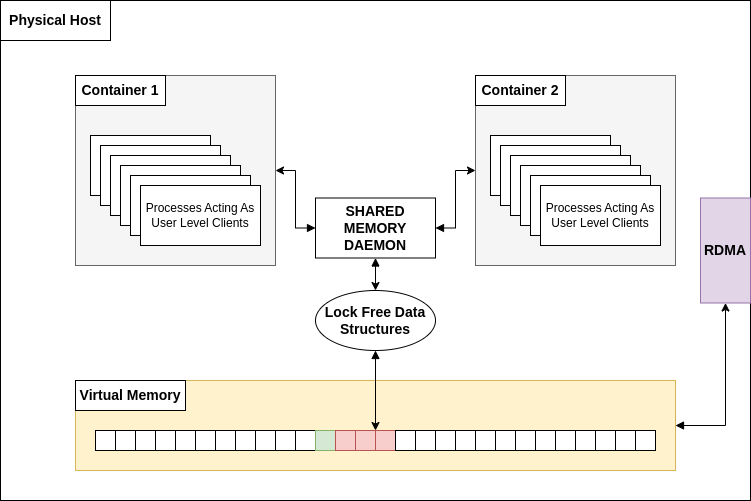
\includegraphics[width=0.8\textwidth]{res3.png}
        \caption{Simple Architecture Of The Proposed Design: User Based}
        \label{fig:desg2}
    \end{figure}
\end{frame}

\begin{frame}
    \frametitle{Test Environment}
    \begin{itemize}
        \item QEMU:
            \begin{itemize}
                \item qemu-system-x86
                \item debootstrap
                \item Bunch of bash scripts
                \item Kernel 6.4.0 with custom configuration (for docker support)
            \end{itemize}
        \item Docker with:
            \begin{itemize}
                \item \textit{-ipc=host}
                \item \textit{-v /dev:/dev}
            \end{itemize}
        \item Simple C++ programs to do the communications.
            \begin{itemize}
                \item One daemon for periodical bookkeeping of the region.
                \item Client program to bookkeep in the first page of the
                    allocated memory.
            \end{itemize}
    \end{itemize}
\end{frame}

\begin{frame}
    \frametitle{Test Environment}
    \begin{figure}
        \centering
        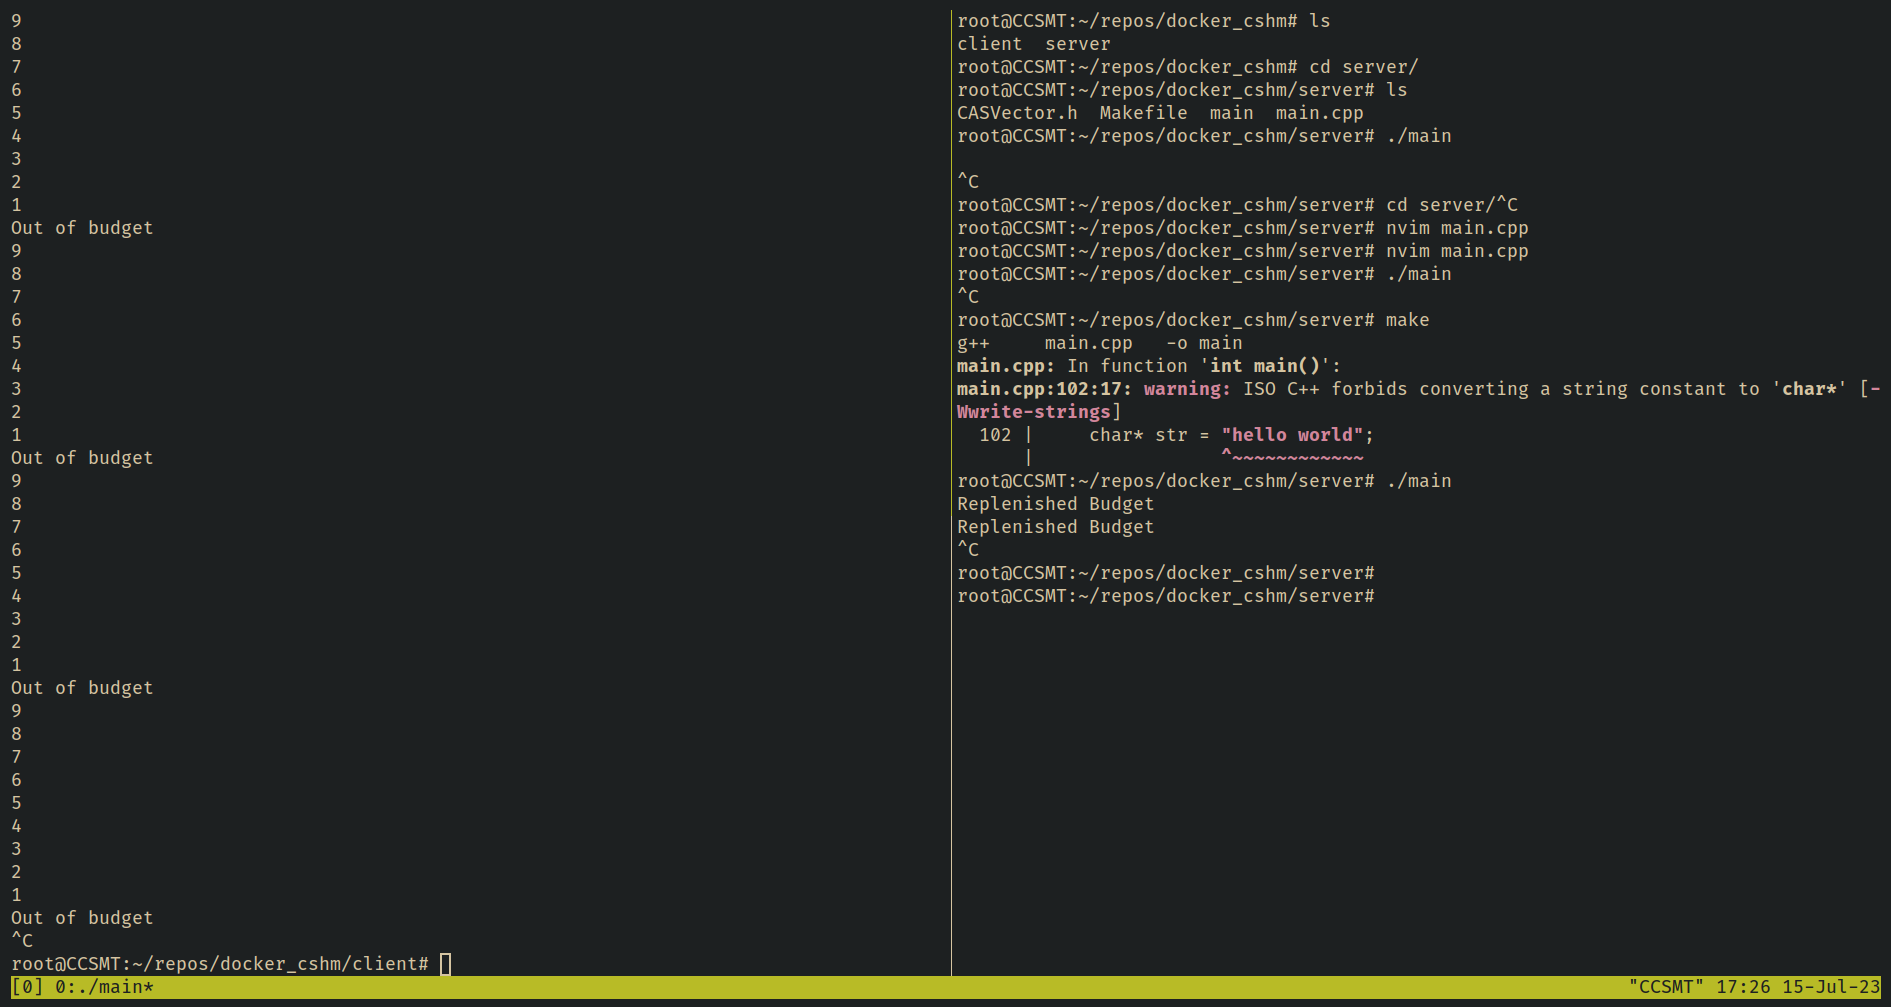
\includegraphics[width=0.8\textwidth]{res2.png}
        \caption{Sample Output of the Daemon Based Desgin}
        \label{fig:res2}
    \end{figure}
\end{frame}

\begin{frame}
    \frametitle{Conclusion and Future Works}
    \begin{itemize}
        \item What We Achieved
            \begin{itemize}
                \item Lock free vector implementation.
                \item User level implementation of the bandwidth manager.
                \item Kernel patch for custom system calls
            \end{itemize}
        \item What Can We Do Next
            \begin{itemize}
                \item Real-time Ethernet.
                \item Handle Serialization and Error Handling.
                \item Handle Heterogeneous machines.
                \item Handle ram access latency via cache coloring and ranks
                    awareness.
                \item Compare the RDMA results with gRPC.
            \end{itemize}
    \end{itemize}
\end{frame}

\begin{frame}
  \centering \Large
  \emph{Thank You For Your Attention}
\end{frame}

\begin{frame}{Reference}
    \bibliographystyle{apalike}
    \bibliography{ref.bib} 
\end{frame}


\end{document}
